\documentclass[12pt,xcolor={rgb}]{beamer}
\usepackage[utf8]{inputenc}
\usepackage[T1]{fontenc}
\usepackage{ngerman}
\usetheme[secheader]{Madrid}


\usepackage {xcolor}
\usepackage{colortbl}
\definecolor {green}{HTML}{04B404}
%\definecolor {red}{HTML}{8A0829}
\definecolor {beige}{HTML}{FFFFFA}
\definecolor {blue}{HTML}{00001E}

\definecolor{UBCblue}{rgb}{0.04706, 0.13725, 0.26667} % UBC Blue (primary)
\usecolortheme[named=UBCblue]{structure}


\begin{document}
\title[Einführung in WebDev B1/T1]{Einführung in Web Development und Shopware Entwicklung}

\subtitle{Block 1 / Teil 1}
\author{Olga Khorkova}

\institute{Sportspar GmbH}
\date{13. August 2019}

\begin{frame}[plain]
\titlepage
\end{frame}


\begin{frame}{Über den Kurs}
\begin{itemize}
\item Anfänger-Niveau
\item Aufgeteilt in 2/(?)3 Blöcke
\item Jeder Block besteht aus 5 Teilen
\item Jeder Block sowie jeder Teil werden mit einem Projekt abgeschlossen 
\item Projekte sowie die Vertiefungsthemen werden gemeinsam abgestimmt
\item Projekte werden reviewed.
\end{itemize}
\end{frame}

\begin{frame}{Über den 1. Block}
\begin{itemize}
\item Web-Arichitektur
\item HTML 5
\item CSS 3
\item PHP/MySQL
\item JavaScript
\item Responsivness
\item SEO, Accessibility, valider Code
\item Architektur von Shopware 5
\item GIT
\item \bf{Abschluss-Projekt B1:} Ein einfaches Shopware-Theme erstellen
\end{itemize}
\end{frame}

\begin{frame}{Über den 2. Block}
\begin{itemize}
\item Vertiefung in CSS
\item Einführung in Preprozessoren (SASS)
\item Einführung in CSS-Frameworks (Bootstrap)
\item Vertiefung in JS
\item JS-Frameworks (jQuery)
\item Web-Animationen
\item Databases
\item Vertiefung in PHP
\item Objekt-Orientierende Programmierung
\item \bf{Abschluss-Projekt B2:} ?
\end{itemize}
\end{frame}


\begin{frame}{Generelle Empfehlungen}
\begin{itemize}
\item Es gibt keine doofe Fragen. 
\item Google is your friend!
\item Macht den Kurs bei Udemy: \textit{Einführung in WebDev}
\item Practice, practice, and practice
\end{itemize}
\end{frame}


\begin{frame}[plain]{Inhalte des 1. Teils}
\tableofcontents
\end{frame}

\section{Web-Architektur}

\begin{frame}{Wie funktioniert Web?}
Generell: web besteht aus zwei Schichten (\textit{tiers})\\

\begin{itemize}
\item Web Browser: präsentiert die Informationen $\rightarrow$ \textbf{Client} 
\item Web Server: liefert die Informationen dem Client $\rightarrow$ \textbf{Server}
\end{itemize}

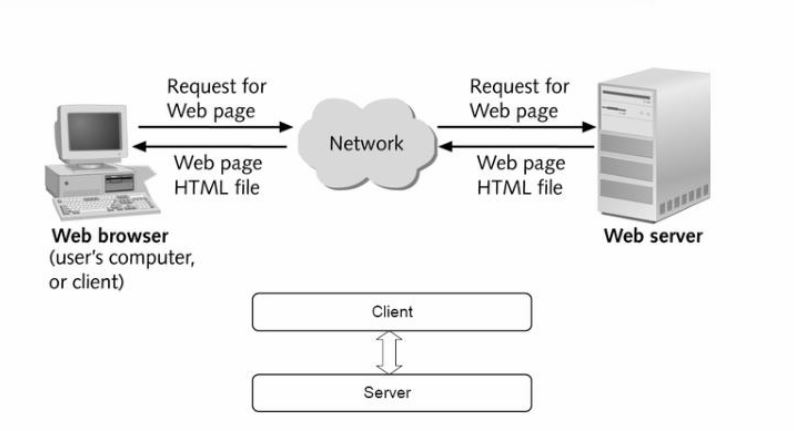
\includegraphics[width=8cm]{imgs/introduction-to-web-architecture.jpg}

\end{frame}

\begin{frame}{Web Server}
Unter dem \textbf{Web Server} wird folgendes verstanden:\\

\begin{itemize}
\item Ein Programm, das HTTP \textit{Requests} akzeptiert und  HTTP \textit{Responses} (\texttt{200}, \texttt{400} etc.) zurückgibt, wobei \textit{data content} optional ist
\item Ein Rechner, der das oben beschriebene Programm ausführt
\end{itemize}

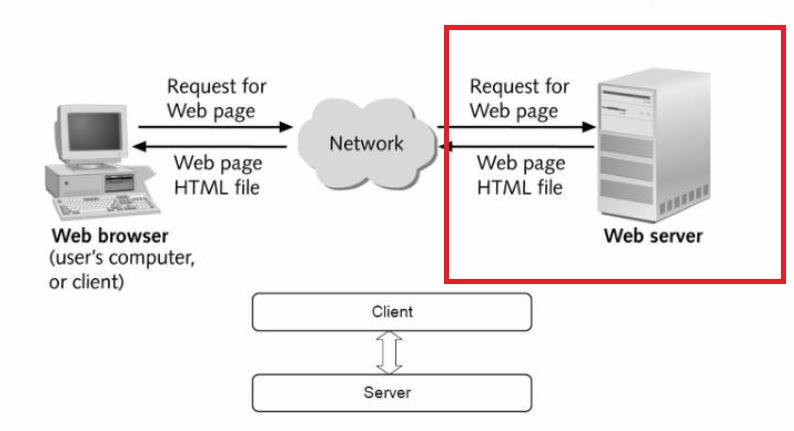
\includegraphics[width=8cm]{imgs/introduction-to-web-architecture_server.jpg}

\end{frame}


\begin{frame}{Client-Server-Modell}
\begin{itemize}
\item Protokoll: \texttt{\color{red}{http}}
\item URL: \texttt{\color{red}{www.sportspar.de}}
\item Repräsentation: \texttt{\color{red}{HTML und CSS}} $\leftarrow$ Thema des 1. Blocks
\end{itemize}

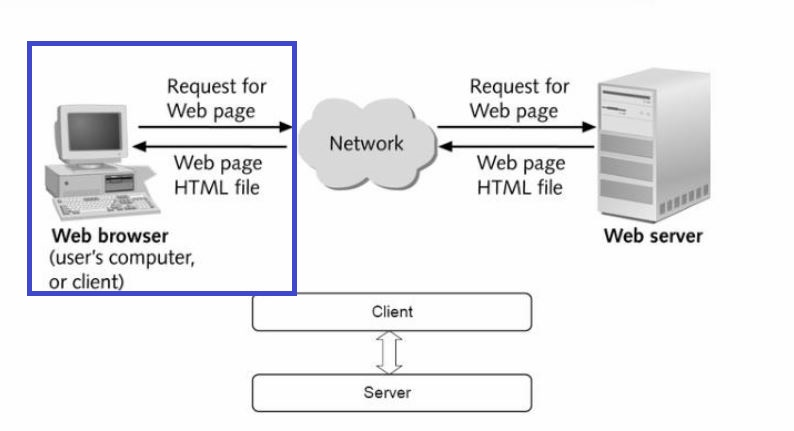
\includegraphics[width=8cm]{imgs/introduction-to-web-architecture_frontend.jpg}
\end{frame}


\section{HTML}

\begin{frame}{HTML}

\Huge\centering{\textbf{HTML}}
\end{frame}

\begin{frame}{HTML Basics 1}
\begin{itemize}
\item es ist keine Programmierspache!!!
\item Hyper Text Markup Language
\end{itemize}
\end{frame}

\begin{frame}{HTML Basics 2}
\begin{itemize}
\item Markup: Darstellen und Positionieren der Elemente auf der Seite. Damit werden Dokumente erzeugt. $\rightarrow$ \textbf{Darstellung}
\item Mit Programmiersprachen werden Scripts oder Programme erstellt, also das, was ausführbar ist. $\rightarrow$ \textbf{Ausführung}
\end{itemize}
\end{frame}


\begin{frame}{index.html}
\texttt{index.html} ist Root-File einer Webseite
\end{frame}

\begin{frame}{Tags Syntax 3 Regeln}
1. \large{\texttt{<irgendeintag>Inhalt</irgendeintag>}}\\
\footnotesize{Der Tag hat immer ein Anfang - \textit{öffnendes tag} und ein Ende - \textit{schliessendes tag}} \\\vspace{0.5cm}
2. \large{\texttt{<u>sehr <b>wichtiger</b> Inhalt</u>}}\\
\footnotesize{Die Tags dürfen ineinadergeschachtelt werden.}\\\vspace{0.5cm}
3. \large{\texttt{<u>sehr <b>wichtiger\color{red}{</u>} Inhalt \color{red}{</b>}}}\\
\footnotesize{Die Tags sollen nicht über Kreuz geschrieben werden.}
\end{frame}


\begin{frame}{visuelle Struktur HTML-Seite}
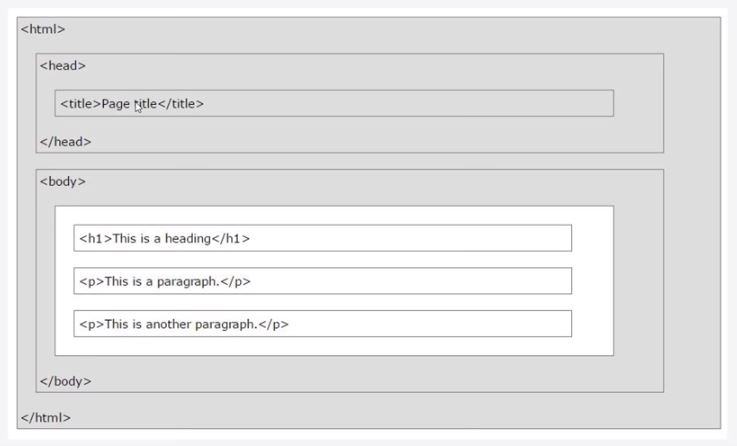
\includegraphics[width=10cm]{imgs/struk_vis.jpg}
\end{frame}

\begin{frame}{Struktur HTML-Seite}
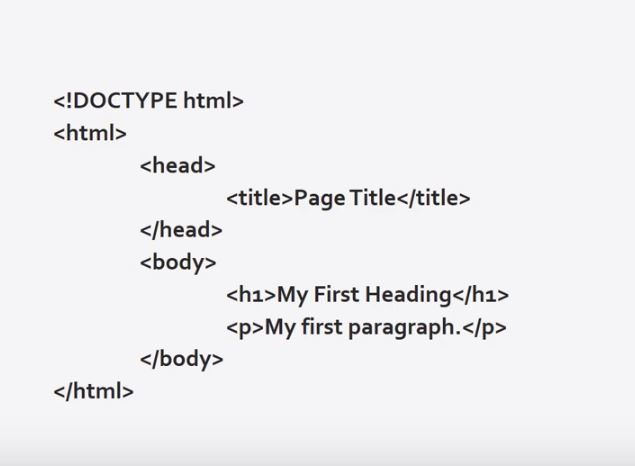
\includegraphics[width=8cm]{imgs/struk_html.jpg}
\end{frame}



\begin{frame}{Tags Attribute 1}
\begin{large}  
{\texttt{<irgendeintag \textcolor{green}{attributename=''attributevalue''}>\\Inhalt</irgendeintag>}}\\
\end{large}
\begin{itemize}
\item Alle Tags können ein Attribut haben
\item Attribute liefern die Informationen über das Element
\item Sie sind in dem öffnenden Tag platziert
\end{itemize}
\end{frame}

\begin{frame}{Tags Attribute 2}
\begin{large}  
\texttt{<p \textcolor{green}{class=''paragraph''}>Inhalt</p>}
\end{large}
\\
\footnotesize{Der gleiche \textit{Class} kann mehreren Elementen zugewiesen werden.}\\
\vspace{0.5cm}
\begin{large}  
\texttt{<p \textcolor{green}{id=''paragraph--special''}>Inhalt</p>}
\end{large}\\
\footnotesize{\textit{ID} darf nur ein Element haben}
\end{frame}


\begin{frame}{Semantik}
Semantische HTML Tags leifern eindeutige Bedeutung der Blöcke sowohl dem Browser als auch dem Developer. Außerdem vereinfacht das das Crawlen der Seite $\rightarrow$ \textbf{SEO}
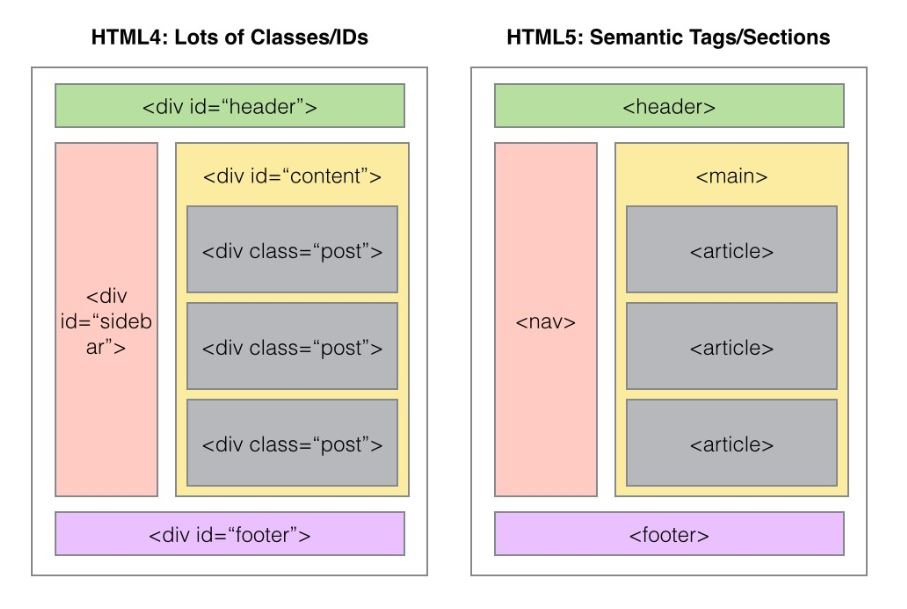
\includegraphics[width=8cm]{imgs/sem_vikigncodeschool.JPG}
\end{frame}


\begin{frame}{Semantik}
\texttt{<header></header>}\\
\texttt{<nav></nav>}\\
\texttt{<main></main>}\\
\texttt{\color{red}{<section></section>}}\\
\texttt{\color{red}{<article></article>}}\\
\texttt{<aside></aside>}\\
\texttt{<footer></footer>}\\
\end{frame}


\begin{frame}{Images}

img ist ein non-binary Tag, d.h. es gibt keinen schliesseneden Tag\\
\vspace{0.5cm}
\texttt{<img src=''https://www.sportspar.de/media/image/15/07/2b/Apple-Icon.png''\\ alt=''apple icon''>}

\end{frame}

\begin{frame}{Links}

\vspace{0.5cm}
\texttt{<a href=''https://www.sportspar.de''></a>}
\end{frame}



\section{CSS}

\begin{frame}{CSS}
\Huge\centering{\textbf{CSS}}
\end{frame}

\begin{frame}{Add CSS}
\begin{itemize}
\item Inline CSS: dierkt in dem HTML-Document $\rightarrow$ \textbf{NO}
\item Internal CSS: <style> Tag direkt in dem Document
\item External CSS: link zu einem css File
\end{itemize}
\end{frame}


\begin{frame}{Basics}
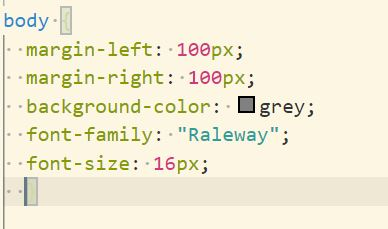
\includegraphics[width=8cm]{imgs/css_basic.JPG} 
\end{frame}


\begin{frame}{Selectoren}
Selectoren: verweisen auf Element, das zu stylen ist. 
\begin{itemize}
\item tag \texttt{\color{green}{h, p, body}}
\item class \texttt{\color{green}{.test--class}}
\item id \texttt{\color{green}{.test--id}}
\end{itemize}
\end{frame}

\begin{frame}{Manche Eigenschaften}
\begin{itemize}
\item margin
\item padding
\item color
\item font-size
\end{itemize}
\end{frame}

\begin{frame}{Kurzschreibweise der Eigenschaften}
Anstatt einzelne Werte für \texttt{margin-top}, \texttt{margin-right}, \texttt{margin-bottom} oder \texttt{margin-left} (bzw. \texttt{padding-…}) anzugeben kann man alle Werte mit in der einen CSS-Eigenschaft \texttt{margin} (bzw. \texttt{padding}) zusammen.\\
\textbf{Die Reihenfolge erfolgt immer im Uhrzeigersinn, angefangen wird beim ...-top Wert.}\\
Die folgenden Schreibweisen sind identisch:
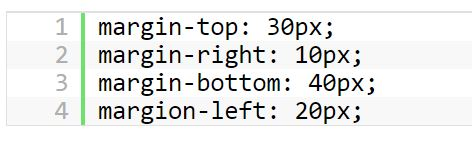
\includegraphics[width=4cm]{imgs/css_lang.JPG}
und 
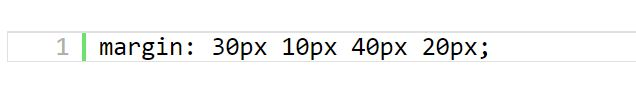
\includegraphics[width=4cm]{imgs/css_kurz.JPG}
\end{frame}


\section{Web Page}

\begin{frame}{Web Page 1}
\begin{itemize}
\item bestehen aus mehreren Files .html, .css, .jpg etc.
\item sind in einem Ordner organisiert
\end{itemize}
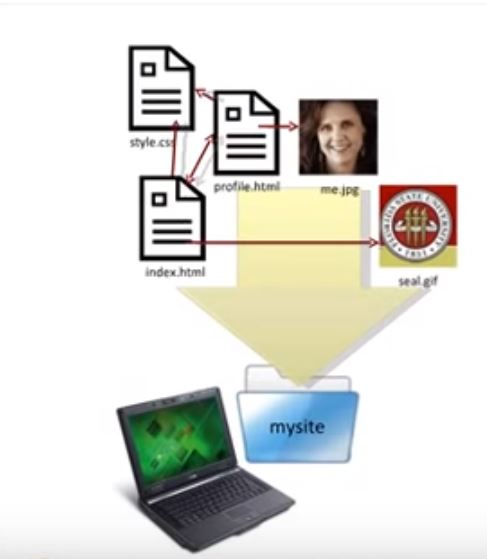
\includegraphics[width=4cm]{imgs/web_page.JPG}
\end{frame}


\begin{frame}{Web Page 2}
\begin{itemize}
\item miteinander verbunden mittels HTML
$\rightarrow$ links zu den relativen Positionen
\item Aufgabe von Browser: alle diese Files miteinander zu verbinden
und die Instruktionen aus dem HTML/CSS zu entnehemen, um zu determinieren,
wie man die Inhalte richtig presenteren muss
\end{itemize}
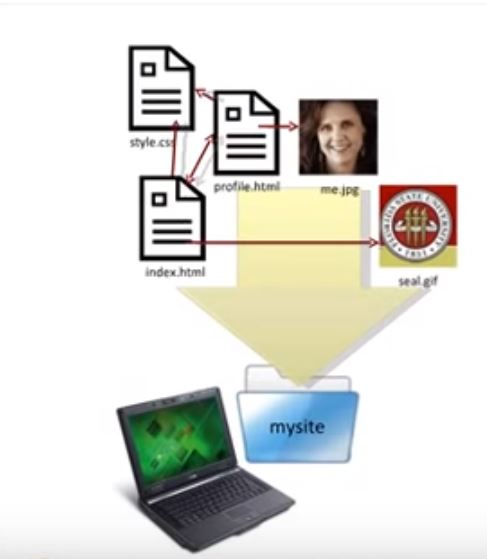
\includegraphics[width=4cm]{imgs/web_page.JPG}
\end{frame}

\section{Zusammenfassung}
\begin{frame}{Zusammenfassung}
\begin{itemize}
\item Client-Server-Model
\item HTML: strukturelle Blöcke des Webs
\item CSS: styling der Blöcke
\item Web Page besteht aus mehreren Files (.html, .css, .jpeg), die auf dem Server liegen und dem Client nach dem Request zur Verfügung gestellt werden.
\end{itemize}
\end{frame}


\section{Aufgabe}
\begin{frame}{Aufgabe}
Es ist eine Aufgabe zu wählen (Struktur und ein wenig CSS ~ Wireframe):
\begin{itemize}
\item Personal Page
\item Layout von Netflix Landing Page nachzubilden
\end{itemize}
\end{frame}

\section{Nützliche Links}

\begin{frame}{Tutorials}
\begin{itemize}
\item Brad Traversy HTML5 \url{https://www.youtube.com/watch?reload=9&v=UB1O30fR-EE}
\item Brad Traversy CSS3 \url{https://www.youtube.com/watch?v=yfoY53QXEnI}
\item w3schools HTML5 \url{https://www.w3schools.com/html/default.asp}
\item w3schools CSS3 \url{https://www.w3schools.com/css/default.asp}
\item HTML Handbook \url{https://www.freecodecamp.org/news/the-html-handbook/}
\end{itemize}
\end{frame}


\begin{frame}{Links}
\begin{itemize}
\item Validator: https://www.w3.org/
\item Editor: VS Code \url{https://code.visualstudio.com/}
\end{itemize}
\end{frame}




\end{document}
%%% Local Variables:
%%% mode: latex
%%% TeX-master: t
%%% End:
